% Options for packages loaded elsewhere
% Options for packages loaded elsewhere
\PassOptionsToPackage{unicode}{hyperref}
\PassOptionsToPackage{hyphens}{url}
\PassOptionsToPackage{dvipsnames,svgnames,x11names}{xcolor}
%
\documentclass[
  letterpaper,
  DIV=11,
  numbers=noendperiod]{scrartcl}
\usepackage{xcolor}
\usepackage{amsmath,amssymb}
\setcounter{secnumdepth}{-\maxdimen} % remove section numbering
\usepackage{iftex}
\ifPDFTeX
  \usepackage[T1]{fontenc}
  \usepackage[utf8]{inputenc}
  \usepackage{textcomp} % provide euro and other symbols
\else % if luatex or xetex
  \usepackage{unicode-math} % this also loads fontspec
  \defaultfontfeatures{Scale=MatchLowercase}
  \defaultfontfeatures[\rmfamily]{Ligatures=TeX,Scale=1}
\fi
\usepackage{lmodern}
\ifPDFTeX\else
  % xetex/luatex font selection
\fi
% Use upquote if available, for straight quotes in verbatim environments
\IfFileExists{upquote.sty}{\usepackage{upquote}}{}
\IfFileExists{microtype.sty}{% use microtype if available
  \usepackage[]{microtype}
  \UseMicrotypeSet[protrusion]{basicmath} % disable protrusion for tt fonts
}{}
\makeatletter
\@ifundefined{KOMAClassName}{% if non-KOMA class
  \IfFileExists{parskip.sty}{%
    \usepackage{parskip}
  }{% else
    \setlength{\parindent}{0pt}
    \setlength{\parskip}{6pt plus 2pt minus 1pt}}
}{% if KOMA class
  \KOMAoptions{parskip=half}}
\makeatother
% Make \paragraph and \subparagraph free-standing
\makeatletter
\ifx\paragraph\undefined\else
  \let\oldparagraph\paragraph
  \renewcommand{\paragraph}{
    \@ifstar
      \xxxParagraphStar
      \xxxParagraphNoStar
  }
  \newcommand{\xxxParagraphStar}[1]{\oldparagraph*{#1}\mbox{}}
  \newcommand{\xxxParagraphNoStar}[1]{\oldparagraph{#1}\mbox{}}
\fi
\ifx\subparagraph\undefined\else
  \let\oldsubparagraph\subparagraph
  \renewcommand{\subparagraph}{
    \@ifstar
      \xxxSubParagraphStar
      \xxxSubParagraphNoStar
  }
  \newcommand{\xxxSubParagraphStar}[1]{\oldsubparagraph*{#1}\mbox{}}
  \newcommand{\xxxSubParagraphNoStar}[1]{\oldsubparagraph{#1}\mbox{}}
\fi
\makeatother


\usepackage{longtable,booktabs,array}
\usepackage{calc} % for calculating minipage widths
% Correct order of tables after \paragraph or \subparagraph
\usepackage{etoolbox}
\makeatletter
\patchcmd\longtable{\par}{\if@noskipsec\mbox{}\fi\par}{}{}
\makeatother
% Allow footnotes in longtable head/foot
\IfFileExists{footnotehyper.sty}{\usepackage{footnotehyper}}{\usepackage{footnote}}
\makesavenoteenv{longtable}
\usepackage{graphicx}
\makeatletter
\newsavebox\pandoc@box
\newcommand*\pandocbounded[1]{% scales image to fit in text height/width
  \sbox\pandoc@box{#1}%
  \Gscale@div\@tempa{\textheight}{\dimexpr\ht\pandoc@box+\dp\pandoc@box\relax}%
  \Gscale@div\@tempb{\linewidth}{\wd\pandoc@box}%
  \ifdim\@tempb\p@<\@tempa\p@\let\@tempa\@tempb\fi% select the smaller of both
  \ifdim\@tempa\p@<\p@\scalebox{\@tempa}{\usebox\pandoc@box}%
  \else\usebox{\pandoc@box}%
  \fi%
}
% Set default figure placement to htbp
\def\fps@figure{htbp}
\makeatother





\setlength{\emergencystretch}{3em} % prevent overfull lines

\providecommand{\tightlist}{%
  \setlength{\itemsep}{0pt}\setlength{\parskip}{0pt}}



 


\KOMAoption{captions}{tableheading}
\makeatletter
\@ifpackageloaded{caption}{}{\usepackage{caption}}
\AtBeginDocument{%
\ifdefined\contentsname
  \renewcommand*\contentsname{Table of contents}
\else
  \newcommand\contentsname{Table of contents}
\fi
\ifdefined\listfigurename
  \renewcommand*\listfigurename{List of Figures}
\else
  \newcommand\listfigurename{List of Figures}
\fi
\ifdefined\listtablename
  \renewcommand*\listtablename{List of Tables}
\else
  \newcommand\listtablename{List of Tables}
\fi
\ifdefined\figurename
  \renewcommand*\figurename{Figure}
\else
  \newcommand\figurename{Figure}
\fi
\ifdefined\tablename
  \renewcommand*\tablename{Table}
\else
  \newcommand\tablename{Table}
\fi
}
\@ifpackageloaded{float}{}{\usepackage{float}}
\floatstyle{ruled}
\@ifundefined{c@chapter}{\newfloat{codelisting}{h}{lop}}{\newfloat{codelisting}{h}{lop}[chapter]}
\floatname{codelisting}{Listing}
\newcommand*\listoflistings{\listof{codelisting}{List of Listings}}
\makeatother
\makeatletter
\makeatother
\makeatletter
\@ifpackageloaded{caption}{}{\usepackage{caption}}
\@ifpackageloaded{subcaption}{}{\usepackage{subcaption}}
\makeatother
\usepackage{bookmark}
\IfFileExists{xurl.sty}{\usepackage{xurl}}{} % add URL line breaks if available
\urlstyle{same}
\hypersetup{
  pdftitle={Selection Bias \& Missing Data Challenge - Part 1},
  colorlinks=true,
  linkcolor={blue},
  filecolor={Maroon},
  citecolor={Blue},
  urlcolor={Blue},
  pdfcreator={LaTeX via pandoc}}


\title{Selection Bias \& Missing Data Challenge - Part 1}
\usepackage{etoolbox}
\makeatletter
\providecommand{\subtitle}[1]{% add subtitle to \maketitle
  \apptocmd{\@title}{\par {\large #1 \par}}{}{}
}
\makeatother
\subtitle{Blue Noise Stippling: Creating Art from Data}
\author{}
\date{}
\begin{document}
\maketitle


\subsection{The Problem: Can Algorithms Create
Art?}\label{the-problem-can-algorithms-create-art}

\textbf{Core Question:} How can we convert a photograph into an
aesthetically pleasing pattern of dots that preserves the visual
information of the original image?

\textbf{The Challenge:} Blue noise stippling is a technique that
converts images into patterns of dots (stipples) using algorithms that
balance visual accuracy with spatial distribution. This challenge asks
you to implement a modified ``void and cluster'' algorithm that combines
importance sampling with blue noise distribution properties to create
stippling patterns that are both visually accurate and spatially
well-distributed.

\textbf{Our Approach:} We'll use a modified void-and-cluster algorithm
that: 1. Creates an importance map identifying visually important
regions 2. Uses a toroidal (periodic) Gaussian kernel for repulsion to
ensure blue noise properties 3. Iteratively selects points with minimum
energy 4. Balances image content importance with blue noise spatial
distribution

\subsection{Introduction to Blue Noise
Stippling}\label{introduction-to-blue-noise-stippling}

Blue noise stippling is a technique for converting images into a pattern
of dots (stipples) that preserves the visual information of the original
image while creating an aesthetically pleasing, evenly distributed
pattern. This method follows the approach described by
\href{https://bartwronski.com/2022/08/31/progressive-image-stippling-and-greedy-blue-noise-importance-sampling/}{Bart
Wronski}.

The method uses a modified ``void and cluster'' algorithm that combines
importance sampling with blue noise distribution properties to create
stippling patterns that are both visually accurate and spatially
well-distributed. This version uses \textbf{smooth extreme
downweighting} that selectively downweights very dark and very light
tones while preserving mid-tones, creating a more balanced distribution
of stipples across the image.

\subsection{Loading the Original
Image}\label{loading-the-original-image}

First, let's load an image that we'll convert to a blue noise stippling
pattern. You can use any image you'd like, but we'll demonstrate with
the provided example.

\begin{figure}[H]

{\centering \pandocbounded{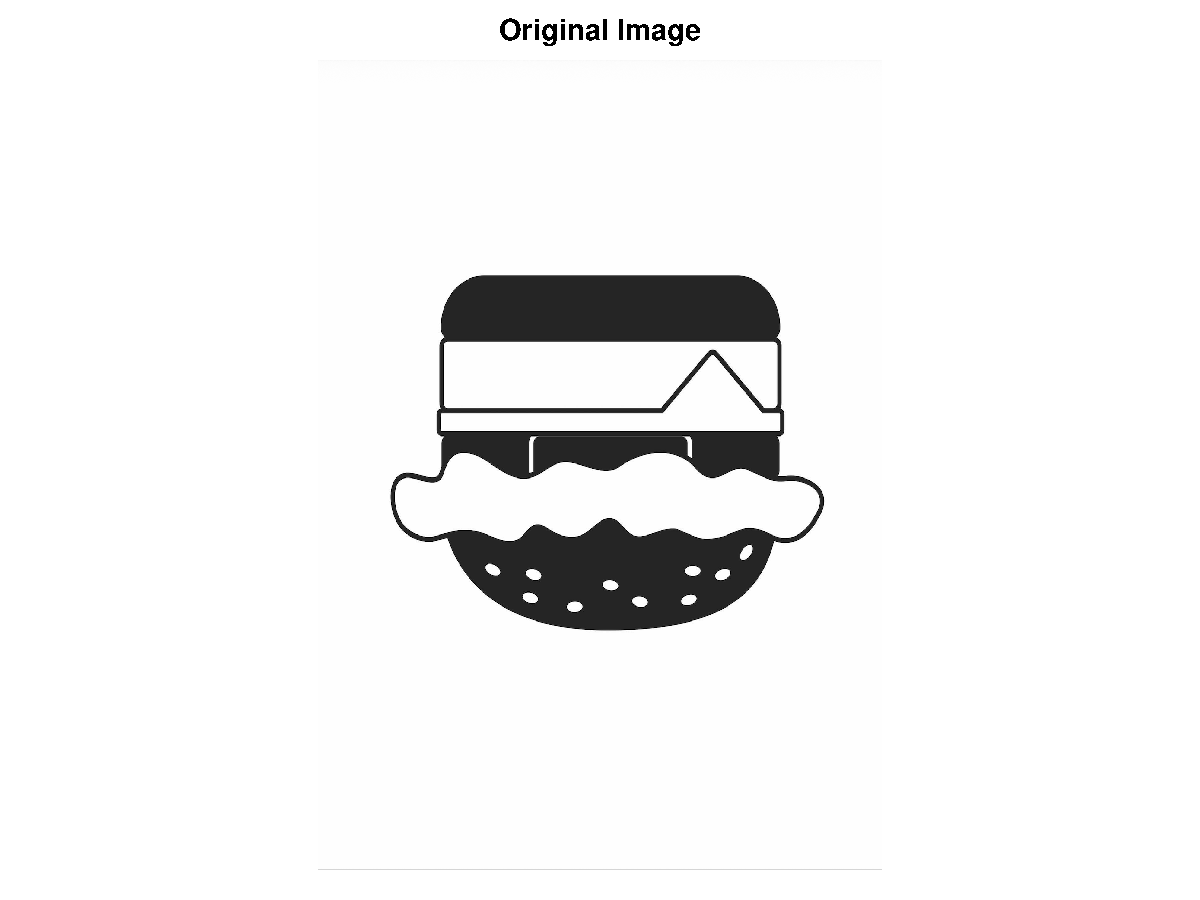
\includegraphics[keepaspectratio]{index_files/figure-pdf/load-image-r-1.pdf}}

}

\caption{Original image before stippling}

\end{figure}%

\begin{verbatim}
Image dimensions: 1564 x 1304 pixels
\end{verbatim}

\subsection{Importance Mapping}\label{importance-mapping}

Before applying the stippling algorithm, we create an \textbf{importance
map} that identifies which regions of the image should receive more
stipples. The importance map is computed by:

\begin{itemize}
\tightlist
\item
  \textbf{Brightness inversion}: The image brightness is inverted so
  that dark areas receive higher importance and thus more dots, while
  light areas receive fewer dots
\item
  \textbf{Extreme tone downweighting}: Smooth Gaussian functions
  downweight tones below 0.2 (very dark) and above 0.8 (very light),
  creating a gradual transition that preserves mid-tones
\item
  \textbf{Mid-tone boost}: A smooth Gaussian function centered on
  mid-tones provides a gradual increase in importance for mid-tone
  regions, ensuring they receive appropriate stippling density
\item
  \textbf{Selective and effective}: This approach ensures that stipples
  are distributed appropriately (more dots in dark areas and mid-tones,
  fewer in extreme dark/light areas) while maintaining good spatial
  distribution
\end{itemize}

\subsection{Blue Noise Stippling
Algorithm}\label{blue-noise-stippling-algorithm}

The stippling algorithm uses a modified void-and-cluster approach that:

\begin{enumerate}
\def\labelenumi{\arabic{enumi}.}
\tightlist
\item
  Creates an importance map that identifies visually important regions
\item
  Initializes an energy field based on the importance map (higher
  importance → lower energy)
\item
  Uses a toroidal (periodic) Gaussian kernel for repulsion to ensure
  blue noise properties
\item
  Iteratively selects points with minimum energy
\item
  Adds Gaussian ``splats'' around selected points to prevent clustering
\item
  Balances image content importance with blue noise spatial distribution
\end{enumerate}

\subsection{Preparing the Working
Image}\label{preparing-the-working-image}

Before generating the stippling pattern, we prepare the image by
resizing if necessary and computing the importance map.

\begin{verbatim}
Resized image to 800 x 667 for processing
\end{verbatim}

\begin{verbatim}
Final image shape: 800 x 667 
\end{verbatim}

\begin{verbatim}
Importance map computed
\end{verbatim}

\subsection{Generating the Stippled
Image}\label{generating-the-stippled-image}

Now let's apply the stippling algorithm to create the blue noise
stippling pattern.

\begin{verbatim}
Generating blue noise stippling pattern...
\end{verbatim}

\begin{verbatim}
Generated 42688 stipple points
\end{verbatim}

\begin{verbatim}
Stipple pattern shape: 800 x 667 
\end{verbatim}

\begin{verbatim}
Saved stippled image to 'stippleImage.rds' (statsMemeChallenge directory not found)
You can manually copy this file to the statsMemeChallenge directory
\end{verbatim}

\subsection{Displaying the Results}\label{displaying-the-results}

Let's visualize the original image, the importance map, and the stippled
version side by side for comparison.

\begin{figure}[H]

{\centering \pandocbounded{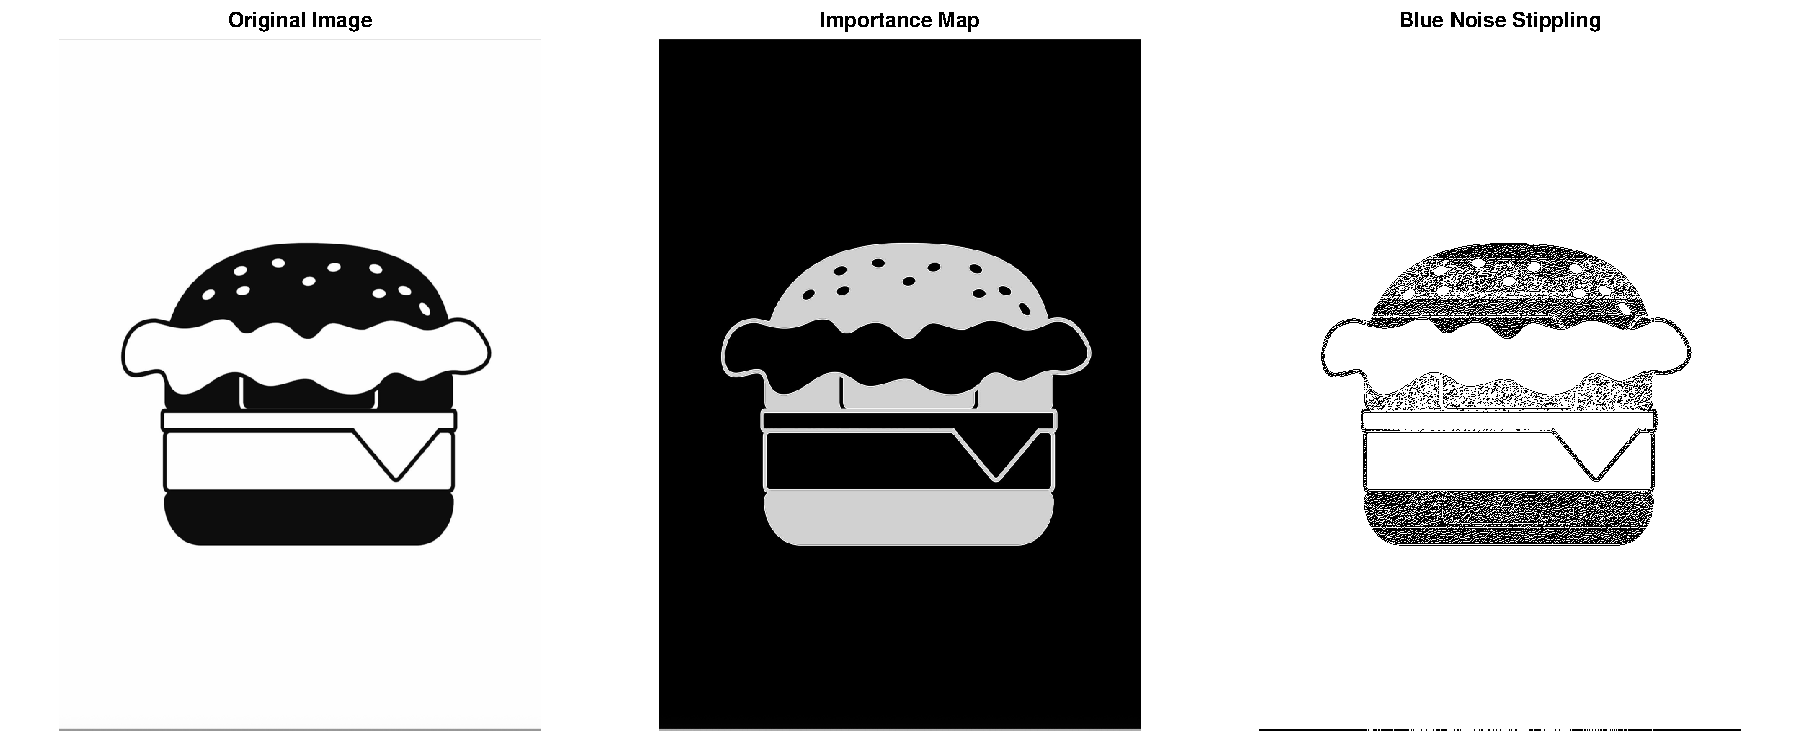
\includegraphics[keepaspectratio]{index_files/figure-pdf/display-results-r-1.pdf}}

}

\caption{Comparison of original image, importance map, and blue noise
stippling}

\end{figure}%

\subsection{Progressive Stippling
Animation}\label{progressive-stippling-animation}

This section creates a GIF showing how the stippled image looks as more
points are added sequentially. We'll use the already-computed stippling
points to generate frames at increments of 100 points.

\begin{verbatim}
Using existing stippling with 42688 points
\end{verbatim}

\begin{verbatim}
Image shape: 800 x 667 
\end{verbatim}

\begin{verbatim}
Generated 428 frames
\end{verbatim}

\begin{verbatim}
Point counts: 1, 100, 200, 300, 400, 500, 600, 700, 800, 900, 1000, 1100, 1200, 1300, 1400, 1500, 1600, 1700, 1800, 1900, 2000, 2100, 2200, 2300, 2400, 2500, 2600, 2700, 2800, 2900, 3000, 3100, 3200, 3300, 3400, 3500, 3600, 3700, 3800, 3900, 4000, 4100, 4200, 4300, 4400, 4500, 4600, 4700, 4800, 4900, 5000, 5100, 5200, 5300, 5400, 5500, 5600, 5700, 5800, 5900, 6000, 6100, 6200, 6300, 6400, 6500, 6600, 6700, 6800, 6900, 7000, 7100, 7200, 7300, 7400, 7500, 7600, 7700, 7800, 7900, 8000, 8100, 8200, 8300, 8400, 8500, 8600, 8700, 8800, 8900, 9000, 9100, 9200, 9300, 9400, 9500, 9600, 9700, 9800, 9900, 10000, 10100, 10200, 10300, 10400, 10500, 10600, 10700, 10800, 10900, 11000, 11100, 11200, 11300, 11400, 11500, 11600, 11700, 11800, 11900, 12000, 12100, 12200, 12300, 12400, 12500, 12600, 12700, 12800, 12900, 13000, 13100, 13200, 13300, 13400, 13500, 13600, 13700, 13800, 13900, 14000, 14100, 14200, 14300, 14400, 14500, 14600, 14700, 14800, 14900, 15000, 15100, 15200, 15300, 15400, 15500, 15600, 15700, 15800, 15900, 16000, 16100, 16200, 16300, 16400, 16500, 16600, 16700, 16800, 16900, 17000, 17100, 17200, 17300, 17400, 17500, 17600, 17700, 17800, 17900, 18000, 18100, 18200, 18300, 18400, 18500, 18600, 18700, 18800, 18900, 19000, 19100, 19200, 19300, 19400, 19500, 19600, 19700, 19800, 19900, 20000, 20100, 20200, 20300, 20400, 20500, 20600, 20700, 20800, 20900, 21000, 21100, 21200, 21300, 21400, 21500, 21600, 21700, 21800, 21900, 22000, 22100, 22200, 22300, 22400, 22500, 22600, 22700, 22800, 22900, 23000, 23100, 23200, 23300, 23400, 23500, 23600, 23700, 23800, 23900, 24000, 24100, 24200, 24300, 24400, 24500, 24600, 24700, 24800, 24900, 25000, 25100, 25200, 25300, 25400, 25500, 25600, 25700, 25800, 25900, 26000, 26100, 26200, 26300, 26400, 26500, 26600, 26700, 26800, 26900, 27000, 27100, 27200, 27300, 27400, 27500, 27600, 27700, 27800, 27900, 28000, 28100, 28200, 28300, 28400, 28500, 28600, 28700, 28800, 28900, 29000, 29100, 29200, 29300, 29400, 29500, 29600, 29700, 29800, 29900, 30000, 30100, 30200, 30300, 30400, 30500, 30600, 30700, 30800, 30900, 31000, 31100, 31200, 31300, 31400, 31500, 31600, 31700, 31800, 31900, 32000, 32100, 32200, 32300, 32400, 32500, 32600, 32700, 32800, 32900, 33000, 33100, 33200, 33300, 33400, 33500, 33600, 33700, 33800, 33900, 34000, 34100, 34200, 34300, 34400, 34500, 34600, 34700, 34800, 34900, 35000, 35100, 35200, 35300, 35400, 35500, 35600, 35700, 35800, 35900, 36000, 36100, 36200, 36300, 36400, 36500, 36600, 36700, 36800, 36900, 37000, 37100, 37200, 37300, 37400, 37500, 37600, 37700, 37800, 37900, 38000, 38100, 38200, 38300, 38400, 38500, 38600, 38700, 38800, 38900, 39000, 39100, 39200, 39300, 39400, 39500, 39600, 39700, 39800, 39900, 40000, 40100, 40200, 40300, 40400, 40500, 40600, 40700, 40800, 40900, 41000, 41100, 41200, 41300, 41400, 41500, 41600, 41700, 41800, 41900, 42000, 42100, 42200, 42300, 42400, 42500, 42600, 42688 
\end{verbatim}

Now let's create the GIF animation:

\begin{figure}[H]

{\centering \pandocbounded{\includegraphics[keepaspectratio]{progressive_stippling.gif}}

}

\caption{Progressive stippling animation showing the sequential build-up
of points. Each frame represents an increment of 100 points,
demonstrating how the blue noise stippling pattern develops as more
points are added.}

\end{figure}%




\end{document}
